\section{Background}
\label{sec:background}


\subsection{LLM Inference and Attention}
LLM inference operates auto-regressively: each output token is generated from the hidden state of the preceding token. Every request passes through two phases. In the \textbf{prefill} phase, all prompt tokens are processed in parallel to produce the first output token; its latency is called \textit{time-to-first-token} (TTFT). In the \textbf{decode} phase, one token is generated per iteration, with per-token latency called \textit{time-between-tokens} (TBT). Prefill is compute-bound due to high token parallelism, while decode is memory-bound due to sequential generation against a growing context.

Each decode step involves three major computations: Self-Attention, Query-Key-Value-Output (QKVO) projection, and a Multi-Layer Perceptron (MLP). Self-attention models global token dependencies as:
\begin{equation}
    \text{Attention}(\mathbf{Q}, \mathbf{K}, \mathbf{V}) = \text{softmax}\left(\frac{\mathbf{Q}\mathbf{K}^T}{\sqrt{d}}\right)\mathbf{V}
\end{equation}
where $d$ is the head dimension. During the decode phase, the query $\mathbf{Q}$ for the current token attends to all prior keys $\mathbf{K}$ and values $\mathbf{V}$. Since $\mathbf{K}$ and $\mathbf{V}$ are reused across steps, they are cached in GPU global memory as the \textbf{KV cache}, eliminating redundant recomputation at the cost of an increasing memory footprint. These two characteristics of LLM inference—the asymmetry between the prefill and decode phases and the memory pressure of the KV cache—motivate much of the systems work discussed below. To delve deeper into this, we first explain how GPUs operate and then present a case study of existing work.

\textcolor{red}{need to add time spent in attention and so on?}

\subsection{GPU Execution Model}
\textcolor{red}{what all things to mention?}
The GPU’s hardware is arranged in a hierarchy that supports execution at a scale of hundreds of thousands of parallel threads. The main processing unit of a GPU is a Streaming Multiprocessor (SM), with modern GPUs containing around a hundred SMs. Each SM has an L1 cache and shared memory, along with tensor cores for accelerated general matrix multiplication (GEMM) and execution units for integer and floating point operations. The shared memory is a user-addressable partition of the L1 cache. The GPU memory is accessed by SMs through the shared L2 cache. \textcolor{red}{mention about prefetcher here, and cite something? Is there some abrupt break in the flow just after this?}


\subsection{Batching and Scheduling for LLM Inference}
A central challenge in LLM serving is that prefill and decode iterations have different compute profiles, making it difficult to mix them in a batch without interference. vLLM~\cite{kwon2023efficient} laid the groundwork for flexible batching by introducing \textit{PagedAttention}, which stores the KV cache in non-contiguous fixed-size memory blocks analogous to virtual memory paging, eliminating fragmentation and enabling KV blocks to be shared across requests. Building on this, Sarathi Serve~\cite{agrawal2024tamingthroughputlatencytradeoffllm} addresses the throughput-latency tradeoff more directly by splitting large prompts into fixed-size chunks via \textit{chunked prefills} and using \textit{stall-free batching} to coalesce these chunks with ongoing decode operations, eliminating the generation stalls caused by long prefill iterations blocking active decodes. Where Sarathi-Serve mitigates interference by interleaving, DistServe~\cite{zhong2024distservedisaggregatingprefilldecoding} eliminates it entirely by disaggregating prefill and decode into separate GPUs, independently optimizing resource allocation and parallelism for each phase. POD-Attention~\cite{Kamath_2025} takes a different approach, keeping both phases on the same GPU while introducing a fused attention kernel with SM-aware CTA scheduling to overlap their compute and memory-bound operations concurrently on the same multiprocessor. Similarly, Bullet~\cite{lin2025boostingllmservingspatialtemporal} exploits spatial-temporal GPU resource sharing between prefill and decode, coupling an SLO-aware scheduler with a dynamic SM resource manager to balance throughput and latency objectives without physical separation. 

Beyond phase co-scheduling, several systems focus on request-level batching policies to improve efficiency. BucketServe~\cite{zheng2025bucketservebucketbaseddynamicbatching} reduces padding waste by grouping requests with similar sequence lengths into buckets, improving GPU memory efficiency. \citet{pang2025optimizing} takes a runtime-adaptive approach, dynamically adjusting batch size based on live GPU memory usage and latency SLA constraints. For offline settings, BlendServe~\cite{zhao2024blendserveoptimizingofflineinference} introduces a resource-aware prefix tree and a dual-scanner scheduling algorithm that reorders and co-schedules requests with complementary compute and memory demands to maximize GPU utilization. Collectively, these works highlight that batching and scheduling decisions, whether at the phase, request, or resource level, have a significant impact on inference efficiency.


\subsection{Prefix Sharing in LLM Serving}
Many real-world workloads, such as few-shot prompting, system prompts, and retrieval-augmented generation (\textcolor{red}{cite for each category, or if done in the intro and not needed here}) involve requests that share a common prompt prefix. Reusing the KV cache of shared prefixes avoids redundant computation and reduces memory pressure, but doing so efficiently requires careful coordination between the serving system and memory management. SGLang~\cite{zheng2024sglangefficientexecutionstructured} was among the first to formalize this, introducing RadixAttention, which uses a radix tree to identify and reuse KV caches across requests with shared prefixes in a multi-call serving setting. Radix trees explicitly store token sequences in a hierarchical structure where common prefixes share the same path. We show a simple example of a radix tree in Figure~\ref{fig:radix_tree_example}.

\begin{figure}[H]
    \centering
    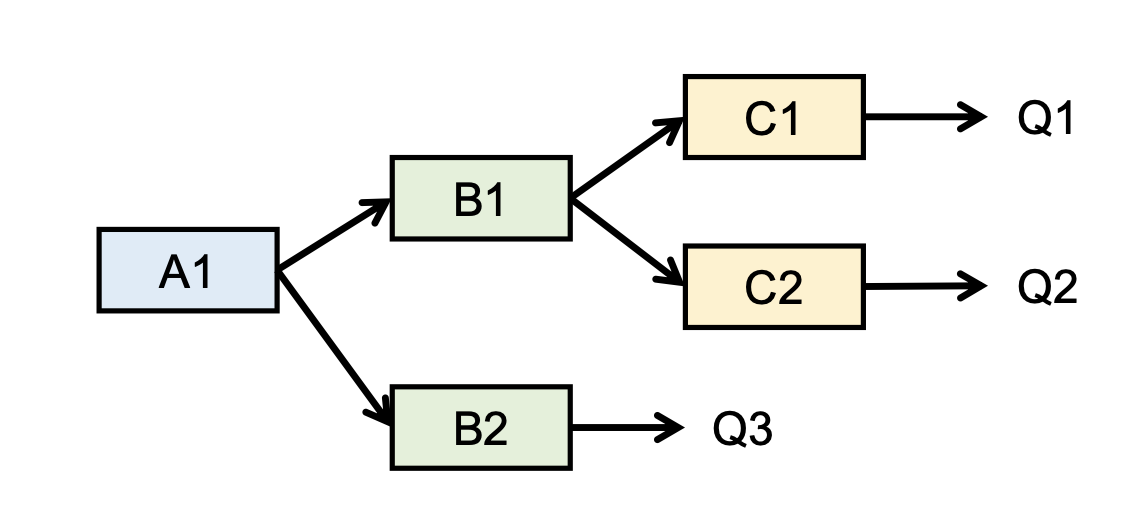
\includegraphics[width=0.8\linewidth]{illustration_images/radix_tree.png}
    \caption{An example of a radix tree from~\cite{MLSYS2025_96894468}, where queries Q1, Q2 share A1, B1 sub-sequences with each other, and only A1 with query Q3.}
    \label{fig:radix_tree_example}
\end{figure}
vLLM~\cite{kwon2023efficient} also implements automatic prefix caching~\cite{vllm_prefix_caching_docs} using a hashing scheme inspired by Merkle trees, as shown in Figure~\ref{fig:vllm_merkle_tree_example}. Each KV-cache block is assigned a hash that depends on both the tokens inside the block and the hash of the preceding prefix block. This effectively forms a chain of hashes representing the entire prefix. If two requests produce the same sequence of hashes, the system can freely reuse the corresponding KV-cache blocks.

\begin{figure}[H]
    \centering
    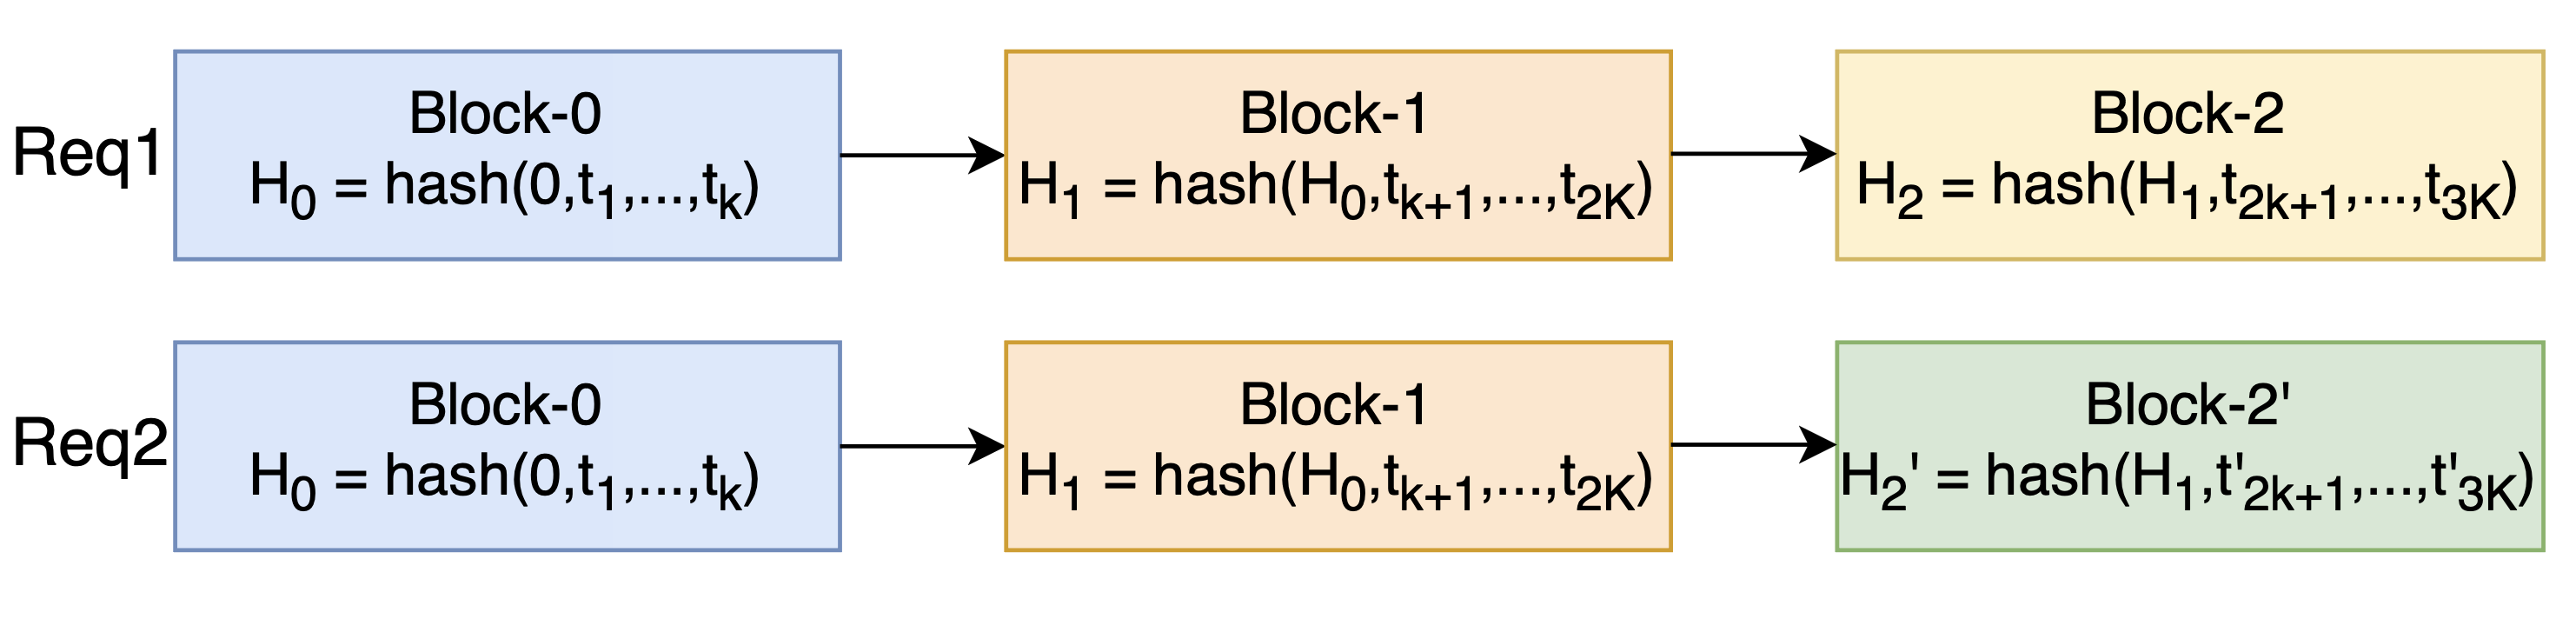
\includegraphics[width=0.8\linewidth]{illustration_images/vllm_merkle_tree.png}
    \caption{An example of vllm Merkle Tree.}
    \label{fig:vllm_merkle_tree_example}
\end{figure}

BatchLLM~\cite{zheng2025batchllmoptimizinglargebatched} extends the idea of prefix sharing to large offline batches, explicitly grouping requests by shared prefixes for global KV cache reuse, then reordering them and applying memory-aware token batching to improve the mix of prefill and decode tokens. BlendServe~\cite{zhao2024blendserveoptimizingofflineinference} similarly leverages a resource-aware prefix tree, but pairs it with a scheduling algorithm that jointly optimizes for both prefix reuse and complementary compute-memory demand balancing. Together, these systems establish that effective prefix sharing requires not just identifying common prefixes but also carefully scheduling the order in which requests are processed to maximize KV cache hit rates and memory efficiency.

\subsection{Prefix-Aware Attention Kernels}
While the systems above handle prefix sharing at the serving and scheduling level, a complementary line of work focuses on exploiting shared prefix structure directly inside the attention kernel, reducing redundant global memory traffic at the GPU execution level. PAT~\cite{yi2025patacceleratingllmdecoding} takes a direct approach by packing queries that share the same prefix into a single CTA, so the shared KV cache is loaded from global memory once and broadcast across all grouped queries. It introduces a pack-forward-merge pipeline with a prefix-aware pack scheduler, multi-tile attention kernels, and multi-stream execution to improve hardware utilization. DEFT~\cite{yao2025deftdecodingflashtreeattention} addresses the same problem in tree-structured decoding by grouping queries according to their shared KV prefixes (KV-guided grouping), ensuring each prefix segment is fetched exactly once; it further introduces Flattened Tree KV Splitting to balance KV partitions across thread blocks for uniform GPU utilization. ChunkAttention~\cite{ye2024chunkattentionefficientselfattentionprefixaware} approaches the problem from a memory layout perspective, storing KV caches in a prefix tree of chunked KV tensors and introducing a two-phase partition kernel, chunk-first and sequence-first, to improve memory locality and parallelism when operating over shared prefix chunks. (\textcolor{red}{improve chunk attention description}) FastTree~\cite{MLSYS2025_96894468} targets radix-tree-structured workloads specifically, grouping queries that share the same tree context to reuse KV cache directly from shared memory, reducing global memory pressure and better utilizing tensor cores. Across all these works, the common insight is that the key to efficient prefix-aware attention lies in restructuring how queries are grouped and how KV data is loaded.

\textcolor{red}{do we need to mention the delta here, or we can skip?}